% Options for packages loaded elsewhere
\PassOptionsToPackage{unicode}{hyperref}
\PassOptionsToPackage{hyphens}{url}
%
\documentclass[
  ignorenonframetext,
  aspectratio=169,
  russian,
]{beamer}
\usepackage{pgfpages}
\setbeamertemplate{caption}[numbered]
\setbeamertemplate{caption label separator}{: }
\setbeamercolor{caption name}{fg=normal text.fg}
\beamertemplatenavigationsymbolshorizontal
% Prevent slide breaks in the middle of a paragraph
\widowpenalties 1 10000
\raggedbottom
\setbeamertemplate{part page}{
  \centering
  \begin{beamercolorbox}[sep=16pt,center]{part title}
    \usebeamerfont{part title}\insertpart\par
  \end{beamercolorbox}
}
\setbeamertemplate{section page}{
  \centering
  \begin{beamercolorbox}[sep=12pt,center]{section title}
    \usebeamerfont{section title}\insertsection\par
  \end{beamercolorbox}
}
\setbeamertemplate{subsection page}{
  \centering
  \begin{beamercolorbox}[sep=8pt,center]{subsection title}
    \usebeamerfont{subsection title}\insertsubsection\par
  \end{beamercolorbox}
}
\AtBeginPart{
  \frame{\partpage}
}
\AtBeginSection{
  \ifbibliography
  \else
    \frame{\sectionpage}
  \fi
}
\AtBeginSubsection{
  \frame{\subsectionpage}
}

\usepackage{amsmath,amssymb}
\usepackage{iftex}
\ifPDFTeX
  \usepackage[T1]{fontenc}
  \usepackage[utf8]{inputenc}
  \usepackage{textcomp} % provide euro and other symbols
\else % if luatex or xetex
  \usepackage{unicode-math}
  \defaultfontfeatures{Scale=MatchLowercase}
  \defaultfontfeatures[\rmfamily]{Ligatures=TeX,Scale=1}
\fi
\usepackage{lmodern}
\usetheme[]{metropolis}
\ifPDFTeX\else  
    % xetex/luatex font selection
\fi
% Use upquote if available, for straight quotes in verbatim environments
\IfFileExists{upquote.sty}{\usepackage{upquote}}{}
\IfFileExists{microtype.sty}{% use microtype if available
  \usepackage[]{microtype}
  \UseMicrotypeSet[protrusion]{basicmath} % disable protrusion for tt fonts
}{}
\usepackage{xcolor}
\newif\ifbibliography
\setlength{\emergencystretch}{3em} % prevent overfull lines
\setcounter{secnumdepth}{-\maxdimen} % remove section numbering

\usepackage{color}
\usepackage{fancyvrb}
\newcommand{\VerbBar}{|}
\newcommand{\VERB}{\Verb[commandchars=\\\{\}]}
\DefineVerbatimEnvironment{Highlighting}{Verbatim}{commandchars=\\\{\}}
% Add ',fontsize=\small' for more characters per line
\usepackage{framed}
\definecolor{shadecolor}{RGB}{241,243,245}
\newenvironment{Shaded}{\begin{snugshade}}{\end{snugshade}}
\newcommand{\AlertTok}[1]{\textcolor[rgb]{0.68,0.00,0.00}{#1}}
\newcommand{\AnnotationTok}[1]{\textcolor[rgb]{0.37,0.37,0.37}{#1}}
\newcommand{\AttributeTok}[1]{\textcolor[rgb]{0.40,0.45,0.13}{#1}}
\newcommand{\BaseNTok}[1]{\textcolor[rgb]{0.68,0.00,0.00}{#1}}
\newcommand{\BuiltInTok}[1]{\textcolor[rgb]{0.00,0.23,0.31}{#1}}
\newcommand{\CharTok}[1]{\textcolor[rgb]{0.13,0.47,0.30}{#1}}
\newcommand{\CommentTok}[1]{\textcolor[rgb]{0.37,0.37,0.37}{#1}}
\newcommand{\CommentVarTok}[1]{\textcolor[rgb]{0.37,0.37,0.37}{\textit{#1}}}
\newcommand{\ConstantTok}[1]{\textcolor[rgb]{0.56,0.35,0.01}{#1}}
\newcommand{\ControlFlowTok}[1]{\textcolor[rgb]{0.00,0.23,0.31}{\textbf{#1}}}
\newcommand{\DataTypeTok}[1]{\textcolor[rgb]{0.68,0.00,0.00}{#1}}
\newcommand{\DecValTok}[1]{\textcolor[rgb]{0.68,0.00,0.00}{#1}}
\newcommand{\DocumentationTok}[1]{\textcolor[rgb]{0.37,0.37,0.37}{\textit{#1}}}
\newcommand{\ErrorTok}[1]{\textcolor[rgb]{0.68,0.00,0.00}{#1}}
\newcommand{\ExtensionTok}[1]{\textcolor[rgb]{0.00,0.23,0.31}{#1}}
\newcommand{\FloatTok}[1]{\textcolor[rgb]{0.68,0.00,0.00}{#1}}
\newcommand{\FunctionTok}[1]{\textcolor[rgb]{0.28,0.35,0.67}{#1}}
\newcommand{\ImportTok}[1]{\textcolor[rgb]{0.00,0.46,0.62}{#1}}
\newcommand{\InformationTok}[1]{\textcolor[rgb]{0.37,0.37,0.37}{#1}}
\newcommand{\KeywordTok}[1]{\textcolor[rgb]{0.00,0.23,0.31}{\textbf{#1}}}
\newcommand{\NormalTok}[1]{\textcolor[rgb]{0.00,0.23,0.31}{#1}}
\newcommand{\OperatorTok}[1]{\textcolor[rgb]{0.37,0.37,0.37}{#1}}
\newcommand{\OtherTok}[1]{\textcolor[rgb]{0.00,0.23,0.31}{#1}}
\newcommand{\PreprocessorTok}[1]{\textcolor[rgb]{0.68,0.00,0.00}{#1}}
\newcommand{\RegionMarkerTok}[1]{\textcolor[rgb]{0.00,0.23,0.31}{#1}}
\newcommand{\SpecialCharTok}[1]{\textcolor[rgb]{0.37,0.37,0.37}{#1}}
\newcommand{\SpecialStringTok}[1]{\textcolor[rgb]{0.13,0.47,0.30}{#1}}
\newcommand{\StringTok}[1]{\textcolor[rgb]{0.13,0.47,0.30}{#1}}
\newcommand{\VariableTok}[1]{\textcolor[rgb]{0.07,0.07,0.07}{#1}}
\newcommand{\VerbatimStringTok}[1]{\textcolor[rgb]{0.13,0.47,0.30}{#1}}
\newcommand{\WarningTok}[1]{\textcolor[rgb]{0.37,0.37,0.37}{\textit{#1}}}

\providecommand{\tightlist}{%
  \setlength{\itemsep}{0pt}\setlength{\parskip}{0pt}}\usepackage{longtable,booktabs,array}
\usepackage{calc} % for calculating minipage widths
\usepackage{caption}
% Make caption package work with longtable
\makeatletter
\def\fnum@table{\tablename~\thetable}
\makeatother
\usepackage{graphicx}
\makeatletter
\newsavebox\pandoc@box
\newcommand*\pandocbounded[1]{% scales image to fit in text height/width
  \sbox\pandoc@box{#1}%
  \Gscale@div\@tempa{\textheight}{\dimexpr\ht\pandoc@box+\dp\pandoc@box\relax}%
  \Gscale@div\@tempb{\linewidth}{\wd\pandoc@box}%
  \ifdim\@tempb\p@<\@tempa\p@\let\@tempa\@tempb\fi% select the smaller of both
  \ifdim\@tempa\p@<\p@\scalebox{\@tempa}{\usebox\pandoc@box}%
  \else\usebox{\pandoc@box}%
  \fi%
}
% Set default figure placement to htbp
\def\fps@figure{htbp}
\makeatother

\IfFileExists{plex-otf.sty}{
  %% Full TeXlive
  % \usepackage[%
  %   % math,
  %   RM={Scale=0.94},SS={Scale=0.94},SScon={Scale=0.94},TT={Scale=MatchLowercase,FakeStretch=0.9},DefaultFeatures={Ligatures=Common}
  % ]{plex-otf}
}{
  %% TinyTeX
  \usepackage{libertine}
}

%%% Load theme
% https://deic.uab.cat/~iblanes/beamer_gallery/
\IfFileExists{beamerthemegotham.sty}{
  %% Full TeXlive
  \usetheme{gotham}
  \gothamset{
    numbering=totalpagenumber,
    parttocframe default=off,
    sectiontocframe default=off,
    subsectiontocframe default=off,
  }
}{
  %% TinyTeX
  \usetheme{Madrid}
}
\makeatletter
\@ifpackageloaded{caption}{}{\usepackage{caption}}
\AtBeginDocument{%
\ifdefined\contentsname
  \renewcommand*\contentsname{Содержание}
\else
  \newcommand\contentsname{Содержание}
\fi
\ifdefined\listfigurename
  \renewcommand*\listfigurename{Список иллюстраций}
\else
  \newcommand\listfigurename{Список иллюстраций}
\fi
\ifdefined\listtablename
  \renewcommand*\listtablename{Список таблиц}
\else
  \newcommand\listtablename{Список таблиц}
\fi
\ifdefined\figurename
  \renewcommand*\figurename{Рисунок}
\else
  \newcommand\figurename{Рисунок}
\fi
\ifdefined\tablename
  \renewcommand*\tablename{Таблица}
\else
  \newcommand\tablename{Таблица}
\fi
}
\@ifpackageloaded{float}{}{\usepackage{float}}
\floatstyle{ruled}
\@ifundefined{c@chapter}{\newfloat{codelisting}{h}{lop}}{\newfloat{codelisting}{h}{lop}[chapter]}
\floatname{codelisting}{Список}
\newcommand*\listoflistings{\listof{codelisting}{Листинги}}
\makeatother
\makeatletter
\makeatother
\makeatletter
\@ifpackageloaded{caption}{}{\usepackage{caption}}
\@ifpackageloaded{subcaption}{}{\usepackage{subcaption}}
\makeatother

\ifLuaTeX
\usepackage[bidi=basic]{babel}
\else
\usepackage[bidi=default]{babel}
\fi
\babelprovide[main,import]{russian}
\babelprovide[import]{english}
% get rid of language-specific shorthands (see #6817):
\let\LanguageShortHands\languageshorthands
\def\languageshorthands#1{}
\usepackage{csquotes}
\usepackage{bookmark}

\IfFileExists{xurl.sty}{\usepackage{xurl}}{} % add URL line breaks if available
\urlstyle{same} % disable monospaced font for URLs
\hypersetup{
  pdftitle={Лабораторная работа №1},
  pdfauthor={Малюга Валерия Васильевна},
  pdflang={ru-RU},
  hidelinks,
  pdfcreator={LaTeX via pandoc}}


\title{Лабораторная работа №1}
\subtitle{Подготовка стенда}
\author{Малюга Валерия Васильевна}
\date{2026-02-21}

\begin{document}
\frame{\titlepage}

\renewcommand*\contentsname{Содержание}
\begin{frame}[allowframebreaks]
  \frametitle{Содержание}
  \setcounter{tocdepth}{1}
  \tableofcontents
\end{frame}

\section{Информация}\label{ux438ux43dux444ux43eux440ux43cux430ux446ux438ux44f}

\begin{frame}{Докладчик}
\phantomsection\label{ux434ux43eux43aux43bux430ux434ux447ux438ux43a}
\begin{columns}[c]
\begin{column}{0.7\linewidth}
\begin{itemize}[<+->]
\tightlist
\item
  Малюга Валерия Васильевна
\item
  студент
\item
  РУДН
\end{itemize}
\end{column}

\begin{column}{0.3\linewidth}
\pandocbounded{\includegraphics[keepaspectratio]{./image/photo.jpg}}
\end{column}
\end{columns}
\end{frame}

\section{Вводная
часть}\label{ux432ux432ux43eux434ux43dux430ux44f-ux447ux430ux441ux442ux44c}

\begin{frame}{Актуальность}
\phantomsection\label{ux430ux43aux442ux443ux430ux43bux44cux43dux43eux441ux442ux44c}
\begin{itemize}[<+->]
\tightlist
\item
  Экспоненциальный рост --- базовая модель в биологии, финансах,
  эпидемиологии
\item
  Литературное программирование повышает воспроизводимость исследований
\item
  Julia + DrWatson + Literate автоматизируют документирование
\end{itemize}
\end{frame}

\begin{frame}{Цель и задачи}
\phantomsection\label{ux446ux435ux43bux44c-ux438-ux437ux430ux434ux430ux447ux438}
\textbf{Цель:} Исследовать модель \(\frac{du}{dt} = \alpha u\)
средствами литературного программирования

\textbf{Задачи:} - Создать структуру проекта по Denote - Реализовать
модель на Julia - Выполнить параметрическое исследование - Сгенерировать
отчет и презентацию
\end{frame}

\section{Выполнение}\label{ux432ux44bux43fux43eux43bux43dux435ux43dux438ux435}

\begin{frame}{Структура проекта}
\phantomsection\label{ux441ux442ux440ux443ux43aux442ux443ux440ux430-ux43fux440ux43eux435ux43aux442ux430}
\begin{figure}[H]

{\centering 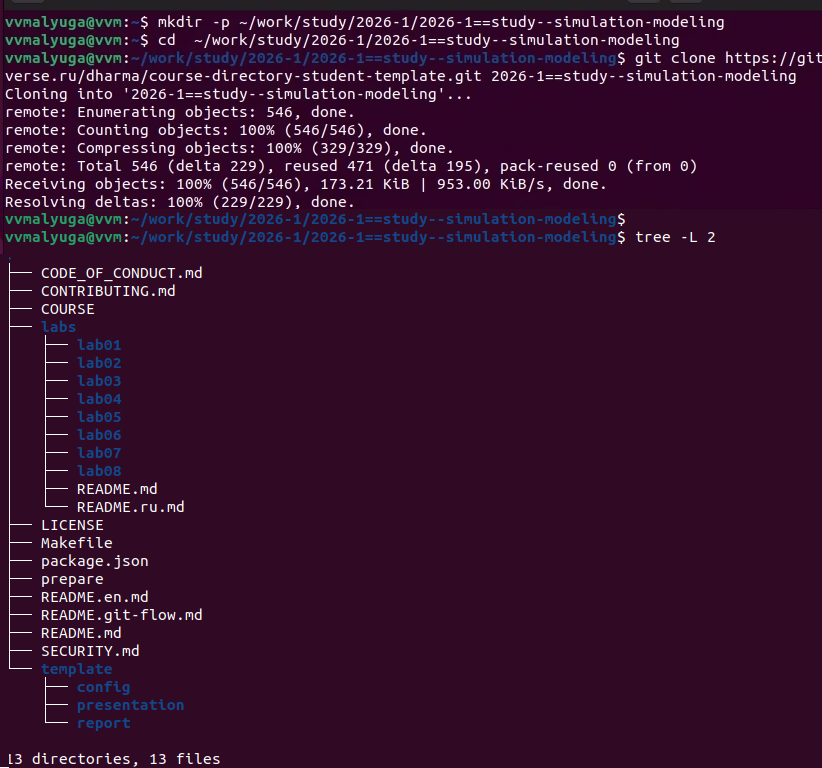
\includegraphics[width=0.8\linewidth,height=\textheight,keepaspectratio]{./image/1.png}

}

\caption{Создание рабочего каталога}

\end{figure}%%
\begin{figure}[H]

{\centering 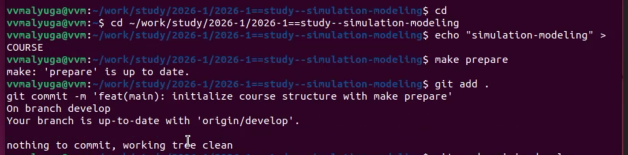
\includegraphics[width=0.8\linewidth,height=\textheight,keepaspectratio]{./image/2.png}

}

\caption{Инициализация курса}

\end{figure}%
\end{frame}

\begin{frame}{Установка пакетов}
\phantomsection\label{ux443ux441ux442ux430ux43dux43eux432ux43aux430-ux43fux430ux43aux435ux442ux43eux432}
\begin{figure}[H]

{\centering 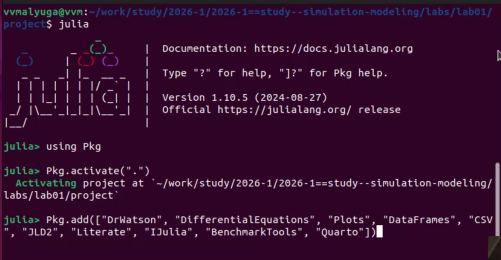
\includegraphics[width=0.8\linewidth,height=\textheight,keepaspectratio]{./image/3.png}

}

\caption{Установка пакетов Julia}

\end{figure}%%
\begin{figure}[H]

{\centering 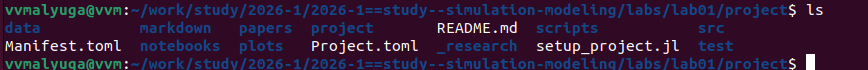
\includegraphics[width=0.8\linewidth,height=\textheight,keepaspectratio]{./image/4.png}

}

\caption{Структура DrWatson}

\end{figure}%
\end{frame}

\begin{frame}[fragile]{Базовая модель}
\phantomsection\label{ux431ux430ux437ux43eux432ux430ux44f-ux43cux43eux434ux435ux43bux44c}
Код модели:

\begin{Shaded}
\begin{Highlighting}[]
\KeywordTok{function} \FunctionTok{exponential\_growth!}\NormalTok{(du, u, p, t)}
\NormalTok{    α }\OperatorTok{=}\NormalTok{ p}
\NormalTok{    du[}\FloatTok{1}\NormalTok{] }\OperatorTok{=}\NormalTok{ α }\OperatorTok{*}\NormalTok{ u[}\FloatTok{1}\NormalTok{]}
\KeywordTok{end}
\end{Highlighting}
\end{Shaded}

Результат: время удвоения = 2.31

\begin{figure}[H]

{\centering 
\includegraphics[width=0.8\linewidth,height=\textheight,keepaspectratio]{../labs/lab01/project/plots/exponential_growth_α=0.3.png}

}

\caption{График экспоненциального роста}

\end{figure}%
\end{frame}

\begin{frame}{Литературный стиль}
\phantomsection\label{ux43bux438ux442ux435ux440ux430ux442ux443ux440ux43dux44bux439-ux441ux442ux438ux43bux44c}
\begin{figure}[H]

{\centering 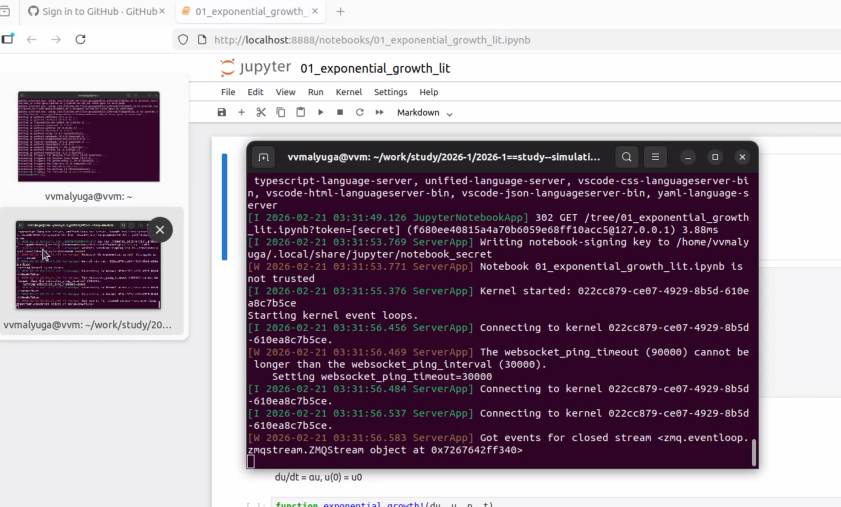
\includegraphics[width=0.8\linewidth,height=\textheight,keepaspectratio]{./image/6.png}

}

\caption{Литературный скрипт с Markdown-разметкой}

\end{figure}%
\end{frame}

\begin{frame}[fragile]{Параметрическое исследование}
\phantomsection\label{ux43fux430ux440ux430ux43cux435ux442ux440ux438ux447ux435ux441ux43aux43eux435-ux438ux441ux441ux43bux435ux434ux43eux432ux430ux43dux438ux435}
Код для набора параметров:

\begin{Shaded}
\begin{Highlighting}[]
\NormalTok{param\_grid }\OperatorTok{=} \FunctionTok{Dict}\NormalTok{(}
    \OperatorTok{:}\NormalTok{α }\OperatorTok{=\textgreater{}}\NormalTok{ [}\FloatTok{0.1}\NormalTok{, }\FloatTok{0.3}\NormalTok{, }\FloatTok{0.5}\NormalTok{, }\FloatTok{0.8}\NormalTok{, }\FloatTok{1.0}\NormalTok{],}
    \OperatorTok{:}\NormalTok{u0 }\OperatorTok{=\textgreater{}}\NormalTok{ [[}\FloatTok{1.0}\NormalTok{]],}
    \OperatorTok{:}\NormalTok{tspan }\OperatorTok{=\textgreater{}}\NormalTok{ [(}\FloatTok{0.0}\NormalTok{, }\FloatTok{10.0}\NormalTok{)]}
\NormalTok{)}
\end{Highlighting}
\end{Shaded}

\begin{figure}[H]

{\centering 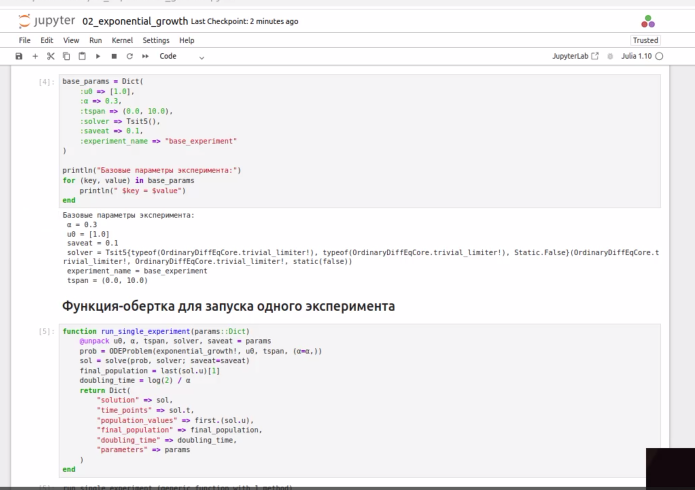
\includegraphics[width=0.8\linewidth,height=\textheight,keepaspectratio]{./image/10.png}

}

\caption{Код параметрического исследования}

\end{figure}%
\end{frame}

\begin{frame}{Результаты}
\phantomsection\label{ux440ux435ux437ux443ux43bux44cux442ux430ux442ux44b}
\begin{longtable}[]{@{}ll@{}}
\toprule\noalign{}
α & Время удвоения \\
\midrule\noalign{}
\endhead
0.1 & 6.93 \\
0.3 & 2.31 \\
0.5 & 1.39 \\
0.8 & 0.87 \\
1.0 & 0.69 \\
\bottomrule\noalign{}
\end{longtable}
\end{frame}

\begin{frame}{График зависимости}
\phantomsection\label{ux433ux440ux430ux444ux438ux43a-ux437ux430ux432ux438ux441ux438ux43cux43eux441ux442ux438}
\begin{figure}[H]

{\centering 
\includegraphics[width=0.9\linewidth,height=\textheight,keepaspectratio]{../labs/lab01/project/plots/02_exponential_growth_params/doubling_time_vs_alpha.png}

}

\caption{Зависимость времени удвоения от α}

\end{figure}%
\end{frame}

\begin{frame}{Генерация артефактов}
\phantomsection\label{ux433ux435ux43dux435ux440ux430ux446ux438ux44f-ux430ux440ux442ux435ux444ux430ux43aux442ux43eux432}
\begin{figure}[H]

{\centering 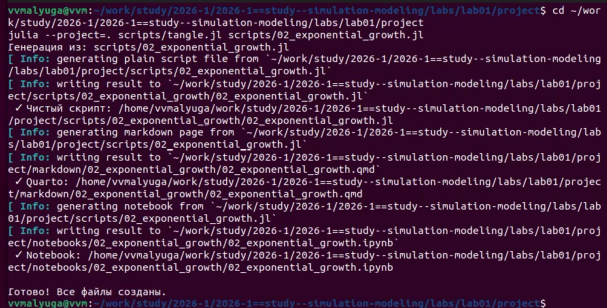
\includegraphics[width=0.8\linewidth,height=\textheight,keepaspectratio]{./image/9.png}

}

\caption{Генерация чистого кода, Jupyter, Quarto}

\end{figure}%
\end{frame}

\begin{frame}{Компиляция отчета}
\phantomsection\label{ux43aux43eux43cux43fux438ux43bux44fux446ux438ux44f-ux43eux442ux447ux435ux442ux430}
\begin{figure}[H]

{\centering 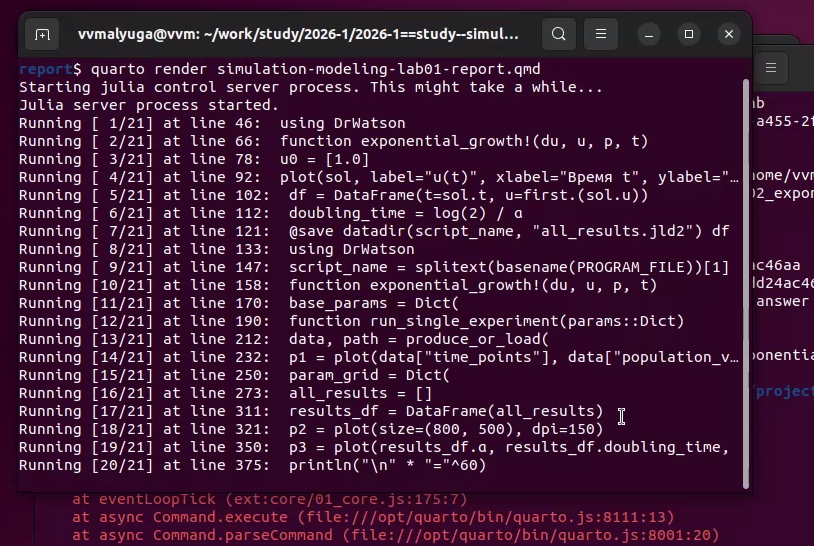
\includegraphics[width=0.8\linewidth,height=\textheight,keepaspectratio]{./image/11.png}

}

\caption{Процесс компиляции Quarto}

\end{figure}%
\end{frame}

\section{Результаты}\label{ux440ux435ux437ux443ux43bux44cux442ux430ux442ux44b-1}

\begin{frame}{Итог}
\phantomsection\label{ux438ux442ux43eux433}
Создано рабочее пространство по Denote\\
Реализована модель на Julia\\
Выполнено параметрическое исследование\\
Применено литературное программирование\\
Сгенерированы отчет и презентация
\end{frame}

\begin{frame}{Главное}
\phantomsection\label{ux433ux43bux430ux432ux43dux43eux435}
\textbf{Модель экспоненциального роста успешно исследована, подтверждена
теоретическая зависимость времени удвоения:} \(T_2 = \ln(2)/\alpha\)
\end{frame}

\section{Ссылки}\label{ux441ux441ux44bux43bux43aux438}

\begin{frame}{Репозитории}
\phantomsection\label{ux440ux435ux43fux43eux437ux438ux442ux43eux440ux438ux438}
\begin{itemize}[<+->]
\tightlist
\item
  GitHub: {[}ссылка{]}
\item
  GitVerse: {[}ссылка{]}
\item
  Релиз v1.0.0: {[}ссылка{]}
\end{itemize}
\end{frame}

\begin{frame}{Скринкасты}
\phantomsection\label{ux441ux43aux440ux438ux43dux43aux430ux441ux442ux44b}
\begin{itemize}[<+->]
\tightlist
\item
  Rutube: {[}ссылка на плейлист{]}
\item
  VKvideo: {[}ссылка на плейлист{]}
\end{itemize}
\end{frame}




\end{document}
